% $Id: template.tex 11 2007-04-03 22:25:53Z jpeltier $

\documentclass{vgtc}                          % final (conference style)
%\documentclass[review]{vgtc}                 % review
%\documentclass[widereview]{vgtc}             % wide-spaced review
%\documentclass[preprint]{vgtc}               % preprint
%\documentclass[electronic]{vgtc}             % electronic version

%% Uncomment one of the lines above depending on where your paper is
%% in the conference process. ``review'' and ``widereview'' are for review
%% submission, ``preprint'' is for pre-publication, and the final version
%% doesn't use a specific qualifier. Further, ``electronic'' includes
%% hyperreferences for more convenient online viewing.

%% Please use one of the ``review'' options in combination with the
%% assigned online id (see below) ONLY if your paper uses a double blind
%% review process. Some conferences, like IEEE Vis and InfoVis, have NOT
%% in the past.

%% Figures should be in CMYK or Grey scale format, otherwise, colour
%% shifting may occur during the printing process.

%% These few lines make a distinction between latex and pdflatex calls and they
%% bring in essential packages for graphics and font handling.
%% Note that due to the \DeclareGraphicsExtensions{} call it is no longer necessary
%% to provide the the path and extension of a graphics file:
%% \includegraphics{diamondrule} is completely sufficient.
%%
\ifpdf%                                % if we use pdflatex
  \pdfoutput=1\relax                   % create PDFs from pdfLaTeX
  \pdfcompresslevel=9                  % PDF Compression
  \pdfoptionpdfminorversion=7          % create PDF 1.7
  \ExecuteOptions{pdftex}
  \usepackage{graphicx}                % allow us to embed graphics files
  \DeclareGraphicsExtensions{.pdf,.png,.jpg,.jpeg} % for pdflatex we expect .pdf, .png, or .jpg files
\else%                                 % else we use pure latex
  \ExecuteOptions{dvips}
  \usepackage{graphicx}                % allow us to embed graphics files
  \DeclareGraphicsExtensions{.eps}     % for pure latex we expect eps files
\fi%

%% it is recomended to use ``\autoref{sec:bla}'' instead of ``Fig.~\ref{sec:bla}''
\graphicspath{{figures/}{pictures/}{images/}{./}} % where to search for the images

\usepackage{microtype}                 % use micro-typography (slightly more compact, better to read)
\PassOptionsToPackage{warn}{textcomp}  % to address font issues with \textrightarrow
\usepackage{textcomp}                  % use better special symbols
\usepackage{mathptmx}                  % use matching math font
\usepackage{times}                     % we use Times as the main font
\renewcommand*\ttdefault{txtt}         % a nicer typewriter font
\usepackage{cite}                      % needed to automatically sort the references

\usepackage{url}            % simple URL typesetting
\usepackage{booktabs}       % professional-quality tables
\usepackage{amsfonts}       % blackboard math symbols
\usepackage{nicefrac}       % compact symbols for 1/2, etc.
\usepackage{microtype}      % microtypography
\usepackage{graphicx}
% \usepackage{eucal}
% \usepackage{breqn}
\usepackage{multicol}
\usepackage{multirow}
\usepackage{capt-of}
% \usepackage{titling}
\usepackage{amsmath}
\usepackage{listings}
\usepackage{siunitx}
%% We encourage the use of mathptmx for consistent usage of times font
%% throughout the proceedings. However, if you encounter conflicts
%% with other math-related packages, you may want to disable it.


%% If you are submitting a paper to a conference for review with a double
%% blind reviewing process, please replace the value ``0'' below with your
%% OnlineID. Otherwise, you may safely leave it at ``0''.
\onlineid{0}

%% declare the category of your paper, only shown in review mode
\vgtccategory{Research}

%% allow for this line if you want the electronic option to work properly
\vgtcinsertpkg

\title{Network Flow Visualization\\CS519: Scientific Visualization (Fall 2021)}

\author{Vincent Chung\thanks{e-mail: vwchung2@illinois.edu}\\ %
     \parbox{1.4in}{\scriptsize \centering Department of\\Computer Science \\ University of Illinois at Urbana-Champaign}}

%% Abstract section.
\abstract{Computer networks facilitate the exchange of vast quantities of information between geographically disparate hosts. In order to optimize large networks for security, quality of service (application latency) and bandwidth utilization, the routing and packet forwarding behaviour of a network are configured and verified by studying flows through the network. In this project, a web-based network flow graph is constructed to visualize IP connection data collected at the Universidad Del Cauca across six days in April and May of 2017 \cite{Rojas:2018:Kaggle}.}

\CCScatlist{
  \CCScatTwelve{Human-centered computing}{Visu\-al\-iza\-tion}{Visu\-al\-iza\-tion techniques}{Treemaps};
  \CCScatTwelve{Human-centered computing}{Visu\-al\-iza\-tion}{Visualization design and evaluation methods}{}
}

\begin{document}

\maketitle

\section{Introduction}

In this project, a web-based network flow graph is constructed to visualize IP connection data collected at the Universidad Del Cauca across six days in April and May of 2017 \cite{Rojas:2018:Kaggle}. An interactive graph of ongoing connections at user-specified points in time are rendered showing the rate and composition of data flows between hosts in the network.

The tool may be extended to be used for any collection of network data flows, presenting active network overlay topologies, and replaying historical events, for example such as day-night traffic and congestion cycles, and DDoS attacks.

The code implementation is organized under the \texttt{dataset/} and \texttt{visualization/} directories for the dataset preprocessing and web visualization portions respectively. These are described in the following sections.

\section{Dataset}

The dataset used for this visualization was collected at the Universidad Del Cauca across six days on 26, 27 and 28 April, and 9, 11 and 15 May of 2017 \cite{Rojas:2018:Kaggle}. It consists of 3,577,296 entries created by the CICFlowMeter tool \cite{cicflowmeter} monitoring a portion of the university's network. The flows are augmented by data from the ntopng tool \cite{ntopng}, which performed Deep Packet Inspection (DPI) on sampled packets to infer the Layer 7 application protocol from the traffic data and flow patterns.

\subsection{Dataset Preprocessing}

To prepare for use by the visualization application, the raw dataset is filtered, sampled and compiled into JSON files to display network flows active at instantaneous timestamps (Fig. \ref{fig:preproc-pipeline}).

\begin{Figure}%[htp]
    \centering
    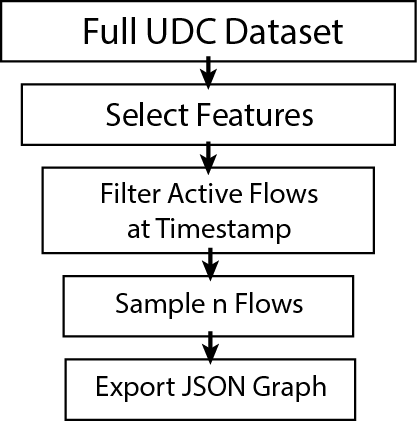
\includegraphics[width=140]{images/cs519-sv_course-project_preprocessing-flow.png}
    \captionof{figure}{The network graph data preprocessing pipeline. }
    \label{fig:preproc-pipeline}
\end{Figure}

Preprocessing is implemented with the \texttt{preproc-data.py} script to generate a JSON network graph at a specific timestamp. The \textt{gen-all-graphs.py} script uses the former to preprocess flow data at six timestamps of interest (morning and evenings) with four quantity of flows, and then generate a manifest file. The quantity of flows chosen is somewhat arbitrary, but are meant to allow the entire graph to fit into conventional web browser displays and fully render the network topology.

\begin{center}
\captionof{table}{List of fields extracted from the Universidad Del Cauca dataset. \cite{Rojas:2018:Kaggle}}
\begin{tabular}{||c | c ||}
    \hline
    \textbf{Attribute} & \textbf{Description} \\
    \hline\hline
    Flow.ID & Unique flow identifier. \\
    Source.IP & Source IPv4 address. \\
    Destination.IP & Destination IPv4 address. \\
    Timestamp & Date and time of flow commencement. \\
    Flow.Duration & Duration of the flow. \\
    Flow.Bytes.s & The average data rate of the flow. \\
    L7Protocol & DPI Layer 7 protocol code. \\
    ProtocolName & DPI Layer 7 protocol name. \\
    \hline
\end{tabular}
\label{tab:dataset-list-fields}
\end{center}

The Python Data Analytics Library (Pandas) \cite{reback2020pandas} is used to ingress and filter the dataset. Out of the 87 features, 8 are extracted (Table \ref{tab:dataset-list-fields}). The flows are then filtered to select only the ones active at the instant of the timestamp (\(T_{inst}\)), using the following:

\begin{equation}
    Flow.Timestamp + Flow.Duration \leq T_{inst}
\end{equation}

Next, the flows are randomly sampled with up to \(n = \{100,300,4000,10000\}\) in each graph. There may be hundreds of thousands of flows active concurrently, which is too many to render in a single graph. Another alternative option would be to perform edge filtering to preserve those links with highest betweeness centrality, but the dataset provides no guarantee that flows form a connected graph, and the removal of the individual edge node flows means that those flows remaining will be aggregates.

Finally, a graph is assembled, the source and destinations become nodes, and their connection becomes edges. Nodes with 3 or more connections is arbitrarily classified as switches. The data rate and protocol information of the flow is embedded in the edge connection.

\section{Network Flow Visualization}

The network visualization is created with the ccNetViz \cite{ccnetviz} library, an interactive graph visualizer with JavaScript bindings. It was chosen for its ability to render using WebGL, which is necessary for performance with large graphs, and customizability.

The graph is hosted as a single-page application, using the Bootstrap \cite{bootstrap} and jQuery \cite{jquery} libraries for layout and interactive controls.

\subsection{Graph Structure}

The network graph has flow terminus as nodes (each labelled with an IPv4 address), and the flow connection as edges. This is not necessarily equivalent to a physical topology (layer 2), as the network can be virtualized. Nodes with 3 or more connections are arbitrarily classified as switches, since most hosts only record a single active flow. This method generally produces good results in this visualization. Switch and host (i.e. client) nodes are shown with different glyphs to distinguish them.

The graph is rendered using the \texttt{force} layout with gravity, charge and friction mechanisms, an algorithm similar or derived from the \textit{Graph drawing by force-directed placement} paper \cite{graph-drawing-force}.

\begin{Figure}%[htp]
    \centering
    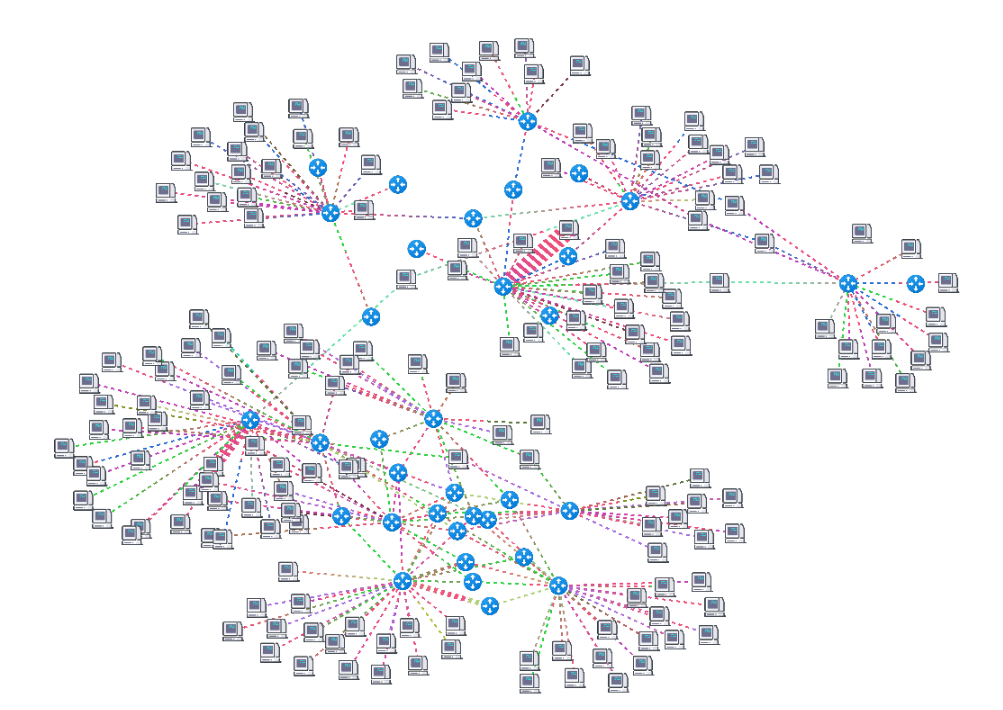
\includegraphics[width=240]{images/cs519-sv_course-project_network-graph.png}
    \captionof{figure}{High-level graph view of network flows between clients and switches.}
    \label{fig:preproc-pipeline}
\end{Figure}

A sliding colour animation in the direction from the source node to the destination node indicates initiating direction of the flow. For example, a client loading a web page would be the source, and the server would be the destination. A server sending a push notification to a client would be the reverse direction. This is used in place of arrows to save screen space, as the large number of connections would inevitably occlude features in high-density regions.

\subsection{Traffic Visualization}

The magnitude of the traffic volume is represented by the width of the edges connecting nodes. The average data rate of the flow relative to the minimum to maximum of the entire sample set is linearly scaled to a value between 1 px and 6 px. Most flows are short-lived, but continuous sessions such as HTTP transfers and video calls will appear as large bands.

\subsection{Traffic Decomposition}

Each flow is augmented with an application-level protocol label from deep packet inspection, unknown and encrypted (with TLS tunneling) flows are opaque however. The protocol code is hashed to produce a pseudo-random RGB colour to label each flow connection edge, and a legend is rendered to allow the use to distinguish between the types of flows. Due to limitations of the graph library however, edge labels and tooltips cannot be rendered, where they would normally display additional context-sensitive details.

\subsection{Interactivity}

The graph visualization may be resized, panned and zoomed to show macro and micro level details of connections, and is performant to several thousand connections. However, this represents only a small fraction of the network activity in the dataset. An possible improvement is to aggregate network flows and its fractional compositions as the region of interest is expanded.

A control is present to select the number of network flows to sample and render, as the number increases, the disparate network subgraphs become connected. A series of labels with timestamps allows the user to select different instances in time to filter the network flows for the graph. This could also have been implemented as a slider with a continuous domain.

Due to technical limitations of the graph library, nodes and edges cannot be dynamically updated without redrawing the entire graph, so both the number of flows and timestamps were preprocessed offline to simplify the implementation. Ideally, a streaming algorithm can play back network flows continuously with low data overhead.

\section{Conclusion}

In this project, a web-based network visualization application was created, drawing network flows active at points in time as edges connecting client and switch nodes. Features such as the direction, magnitude and the composition of the flow are shown a visual properties, and interactive UI elements allow the number of flows and time attribute to be controlled.

The visualization my be improved by writing a custom graph renderer and data streaming backend that is not limited by programming model and extensibility of general purpose ones.

%\bibliographystyle{abbrv}
% \bibliographystyle{abbrv-doi}
%\bibliographystyle{abbrv-doi-narrow}
%\bibliographystyle{abbrv-doi-hyperref}
%\bibliographystyle{abbrv-doi-hyperref-narrow}

\bibliographystyle{IEEEtran}
\bibliography{references}

\end{document}
